\chapter{Psalm 72}

\begin{figure}
  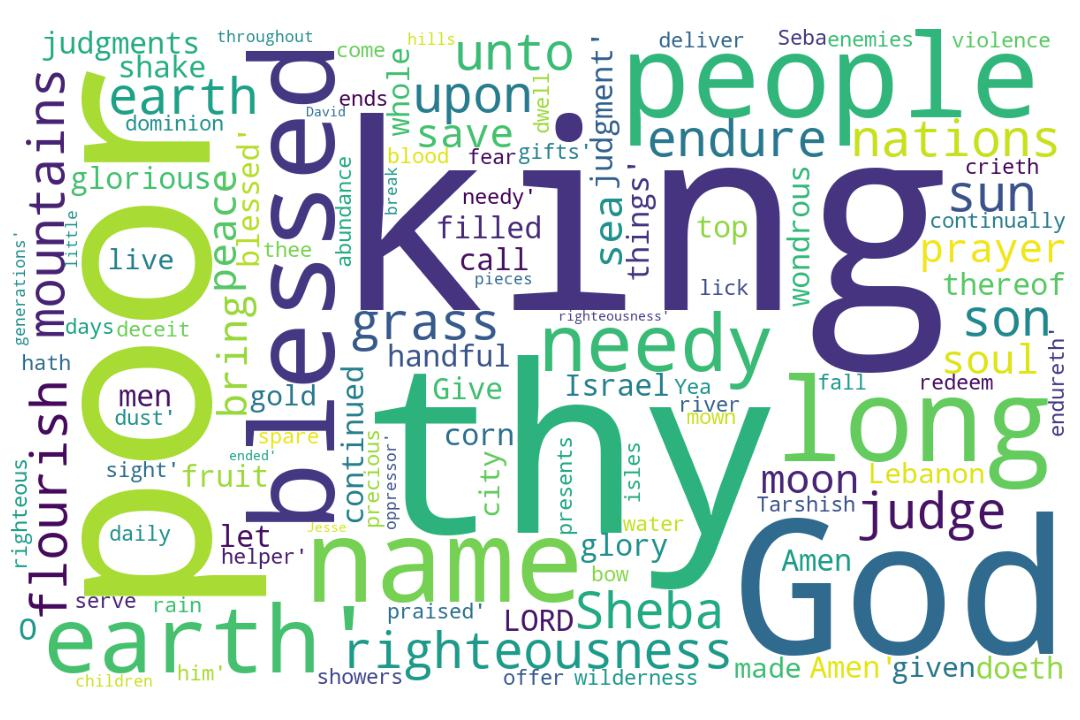
\includegraphics[width=\linewidth]{19OT-Psalms/Psalm72-WordCloud.jpg}
  \caption{Psalm 72 Word Cloud}
  \label{fig:Psalm 72 word Cloud}
\end{figure}


\marginpar{\scriptsize \centering \fcolorbox{bone}{lime}{\textbf{WITH THE PRINCE OF PEACE}}\\ (Psalm 72) \begin{compactenum}[I.][8]
    \item \textbf{Perfection in Judgment} \index[scripture]{Psalms!Psa 072:02}(Psa 72:2)
    \item The \textbf{Poor Blessed} \index[scripture]{Psalms!Psa 072:04}(Psa 72:4)
    \item \textbf{Peace Finally Arrives} \index[scripture]{Psalms!Psa 072:07}(Psa 72:7)
    \item \textbf{Opponents Praising} \index[scripture]{Psalms!Psa 072:09, 10}(Psa 72:9, 10)
    \item \textbf{Politics Centered on the Lord} \index[scripture]{Psalms!Psa 072:11}(Psa 72:11)
    \item \textbf{Produce Incredible} \index[scripture]{Psalms!Psa 072:16}(Psa 72:16)
    \item \textbf{Praise Continual} \index[scripture]{Psalms!Psa 072:17}(Psa 72:17)
\end{compactenum}}



\footnote{\textcolor[cmyk]{0.99998,1,0,0}{\hyperlink{TOC}{Return to end of Table of Contents.}}}\footnote{\href{https://audiobible.com/bible/psalms_72.html}{\textcolor[cmyk]{0.99998,1,0,0}{Psalm 72 Audio}}}\textcolor[cmyk]{0.99998,1,0,0}{\emph{A Psalm} for Solomon.}\\
\\
\textcolor[cmyk]{0.99998,1,0,0}{Give the king thy judgments, O God, and thy \fcolorbox{bone}{MYGOLD}{righteousness} unto the king's son.}
[2] \textcolor[cmyk]{0.99998,1,0,0}{He shall \fcolorbox{bone}{lime}{judge} thy people with \fcolorbox{bone}{MYGOLD}{righteousness}, and thy poor with judgment.}
[3] \textcolor[cmyk]{0.99998,1,0,0}{The mountains shall bring peace to the people, and the little hills, by \fcolorbox{bone}{MYGOLD}{righteousness}.}
[4] \textcolor[cmyk]{0.99998,1,0,0}{He shall judge the \fcolorbox{bone}{lime}{poor} of the people, he shall save the children of the needy, and shall break in pieces the oppressor.}
[5] \textcolor[cmyk]{0.99998,1,0,0}{They shall fear thee as long as the sun and moon endure, throughout all generations.}
[6] \textcolor[cmyk]{0.99998,1,0,0}{He shall come down like rain upon the mown grass: as showers \emph{that} water the earth.}
[7] \textcolor[cmyk]{0.99998,1,0,0}{In his days shall the righteous flourish; and abundance of \fcolorbox{bone}{lime}{peace} so long as the moon endureth.}
[8] \textcolor[cmyk]{0.99998,1,0,0}{He shall have dominion also from sea to sea, and from the river unto the ends of the earth.}\footnote{\textbf{Psalm 145:13} - Thy kingdom is an everlasting kingdom, and thy dominion endureth throughout all generations.}\footnote{\textbf{Zechariah 9:10} - And I will cut off the chariot from Ephraim, and the horse from Jerusalem, and the battle bow shall be cut off: and he shall speak peace unto the heathen: and his dominion shall be from sea even to sea, and from the river even to the ends of the earth.}\footnote{\textbf{Revelation 1:6} - And hath made us kings and priests unto God and his Father; to him be glory and dominion for ever and ever. Amen.}
[9] \textcolor[cmyk]{0.99998,1,0,0}{They that dwell in the wilderness shall \fcolorbox{bone}{lime}{bow before him}; and his enemies shall lick the dust.}
[10] \textcolor[cmyk]{0.99998,1,0,0}{The kings of Tarshish and of the isles shall bring presents: the kings of Sheba and Seba shall offer gifts.}
[11] \textcolor[cmyk]{0.99998,1,0,0}{Yea, all kings shall fall down \fcolorbox{bone}{lime}{before him}: all nations shall serve him.}
[12] \textcolor[cmyk]{0.99998,1,0,0}{For he shall deliver the needy when he crieth; the poor also, and \emph{him} that hath no helper.}
[13] \textcolor[cmyk]{0.99998,1,0,0}{He shall spare the poor and needy, and shall save the souls of the needy.}
[14] \textcolor[cmyk]{0.99998,1,0,0}{He shall redeem their soul from deceit and violence: and precious shall their blood be in his sight.}
[15] \textcolor[cmyk]{0.99998,1,0,0}{And he shall live, and to him shall be given of the gold of Sheba: prayer also shall be made for him continually; \emph{and} daily shall he be praised.}\footnote{\textbf{1 Kings 10:1-13} - And when the queen of Sheba heard of the fame of Solomon concerning the name of the LORD, she came to prove him with hard questions. [2] And she came to Jerusalem with a very great train, with camels that bare spices, and very much gold, and precious stones: and when she was come to Solomon, she communed with him of all that was in her heart. [3] And Solomon told her all her questions: there was not any thing hid from the king, which he told her not. [4] And when the queen of Sheba had seen all Solomon’s wisdom, and the house that he had built, [5] And the meat of his table, and the sitting of his servants, and the attendance of his ministers, and their apparel, and his cupbearers, and his ascent by which he went up unto the house of the LORD; there was no more spirit in her. [6] And she said to the king, It was a true report that I heard in mine own land of thy acts and of thy wisdom. [7] Howbeit I believed not the words, until I came, and mine eyes had seen it: and, behold, the half was not told me: thy wisdom and prosperity exceedeth the fame which I heard. [8] Happy are thy men, happy are these thy servants, which stand continually before thee, and that hear thy wisdom. [9] Blessed be the LORD thy God, which delighted in thee, to set thee on the throne of Israel: because the LORD loved Israel for ever, therefore made he thee king, to do judgment and justice. [10] And she gave the king an hundred and twenty talents of gold, and of spices very great store, and precious stones: there came no more such abundance of spices as these which the queen of Sheba gave to king Solomon. [11] And the navy also of Hiram, that brought gold from Ophir, brought in from Ophir great plenty of almug trees, and precious stones. [12] And the king made of the almug trees pillars for the house of the LORD, and for the king’s house, harps also and psalteries for singers: there came no such almug trees, nor were seen unto this day. [13] And king Solomon gave unto the queen of Sheba all her desire, whatsoever she asked, beside that which Solomon gave her of his royal bounty. So she turned and went to her own country, she and her servants.}\footnote{\textbf{Isaiah 60:6} - The multitude of camels shall cover thee, the dromedaries of Midian and Ephah; all they from Sheba shall come: they shall bring gold and incense; and they shall shew forth the praises of the LORD.}
[16] \textcolor[cmyk]{0.99998,1,0,0}{There shall be an handful of corn in the earth upon the top of the mountains; the \fcolorbox{bone}{lime}{fruit} thereof shall shake like Lebanon: and \emph{they} of the city shall flourish like grass of the earth.}
[17] \textcolor[cmyk]{0.99998,1,0,0}{His name shall endure for ever: his name shall be \fcolorbox{bone}{lime}{continued} as long as the sun: and \emph{men} shall be blessed in him: all nations shall call him blessed.}
[18] \textcolor[cmyk]{0.99998,1,0,0}{Blessed \emph{be} the LORD God, the God of Israel, who only doeth wondrous things.}
[19] \textcolor[cmyk]{0.99998,1,0,0}{And blessed \emph{be} his glorious name for ever: and let the whole earth be filled \emph{with} his glory; Amen, and Amen.}
[20] \textcolor[cmyk]{0.99998,1,0,0}{The prayers of David the son of Jesse are ended.}

